--Explain the tool from a high-level point of view--

This work presents  \toolName\ (Multi-robot plAnner for PArtially Known EnviRonments), a \emph{novel} \emph{decentralized} planner for partially known environments.
\toolName\ modifies~\cite{tumova2016multi} by supporting partial knowledge.
This tool splits the given set of robot that conforms the team into classes depending on the local mission that each of them must achieve.
Then, the planner computes possible and definitive plans based on the model of the environment and its partial knowledge.
A \emph{definitive plan} is a sequence of actions that ensure the satisfaction of the local mission for each robot. 
A \emph{possible plan} is a sequence of actions that may satisfy the local mission due to some unknown information about the model of the robots or the environment in which they are deployed. 
If \toolName is able to find a plan, it is performed in order to achieve each robot's mission.
The tool always try to reach the goal performing the lower number of actions.

Each robot is able to perform a complex mission, therefor the goals that they reach in the environment represent points where a service is provided \sergio{reference to the other paper containing the running example?} or where two robots can synchronize.
However, in order to reach these goals robots must face different issues related with partial knowledge, as listed in the following lines.

\textbf{Partial knowledge about the actions execution.} 
The transition between two of the cells that conform the grid map of the environment can be:
\begin{enumerate*}
\item always possible;
\item always not possible (i.e. a wall);
\item not known (i.e. a door between two rooms that can be open or closed).
\end{enumerate*}
\toolName is able to compute a plan that goes through an unknown transition, therefor performing a \emph{possible plan}.

\textbf{Unknown service provisioning.} 
In the dynamic environments studied for this work whether a service is provided or not in a specific location could be unknown. \sergio{reference to the other paper containing the running example?}
In order to achieve the mission with the minimum number of actions performed, \toolName~ is able to compute a plan that tries to reach an uncertain service.
Thus, \toolName~ computes a \emph{possible plan}.

\textbf{Unknown meeting capabilities.} 
As stated before, robots can meet and synchronize in certain locations.
There they can perform a mission, as exchanging a load, in a collaborative fashion.\sergio{reference to the other paper containing the running example?}
In this case, two or more robots that are part of the same subset part of the whole team can compute a plan whose goal is to meet in an uncertain synchronization point.
Thus, \toolName computes a \emph{possible plan}.

Whenever a robot approaches to an location with uncertain information, it detects if this transition, service, or meeting capability is detected to be firable, provided, and possible, respectively.
The robot then updates the information concerning to this location, setting it yo ``true" or ``false".
This information is shared with the rest of the team so it can be take into account for further planning.

An overview of \toolName\ is depicted in ~\ref{fig:overview}.
The \emph{Planner} script uses the models of the robot(s) and the environment in order to compute the path-planning.
The model of each robot contains information regarding its initial position, the number of services that the robot must perform and their location and the locations where the modeled robot has to synchronize with another one.  
The model of the environment represents its map and defines the allowance of transitions between the cells that compound the model (i.e. walls). 
This two models must be manually defined but can be reused for an infinite number of experiments.
Then, the \emph{Random model generator} generates a certain number (defined by the user) of tests based on the previously explained models.
Each of this tests is unique since the generator associates a random uncertainty and an initial position of the robotic team to each of them.
This process is automatically performed for each experiment, since the uncertainty that is checked changes between them (e.g. execution of transitions in \emph{Experiment 1}, services provisioning in \emph{Experiment 2} and meeting capabilities in \emph{Experiment 3}).
The generation of models must be performed once, although we provide an already working set in our repository and this step can be skipped.
The already existing models of the environment represent models of real robot applications, i.e., the RoboCup Logistics League competition~\cite{karrasrobocup} and an apartment of a large residential facility for senior citizens~\cite{map}.
This set is stored in the folder "ReplicationPackage", where the new scenarios must be saved as well.

Once the models are set, the planner can be executed selecting the number of experiment to perform and the research question to be checked.
The approach that is followed in order to test the uncertainty of the environment and its repercussion into the performance of the tool is explained in the following.

Step 1. For the first step a partial model of the whole robot application is loaded. 
~\toolName~ then computes a \emph{possible plan}, which is executed by the robot(s).
When executing the plan, every time a robot detects a false evidence about a partial information , e.g., a transition of the plan is not executable, \toolName~ is re-executed to recompute a new \emph{possible plan}.

Step 2. For this case all the unknown information regarding the robotic application is set to false, meaning that \toolName~ will always return a \emph{definitive plan}.

During the performance of the two steps for a certain number of experiments \toolName~ collects information regarding:
\begin{enumerate*}
\item the length of each plan;
\item the time that took to the tool to compute each plan;
\item the ratio between the length of definitive and possible plans;
\item the ratio between the time expect computing definitive and possible plans;
\item the false and true evidences found during execution.
\end{enumerate*}

\begin{figure}[!t]
\begin{center}
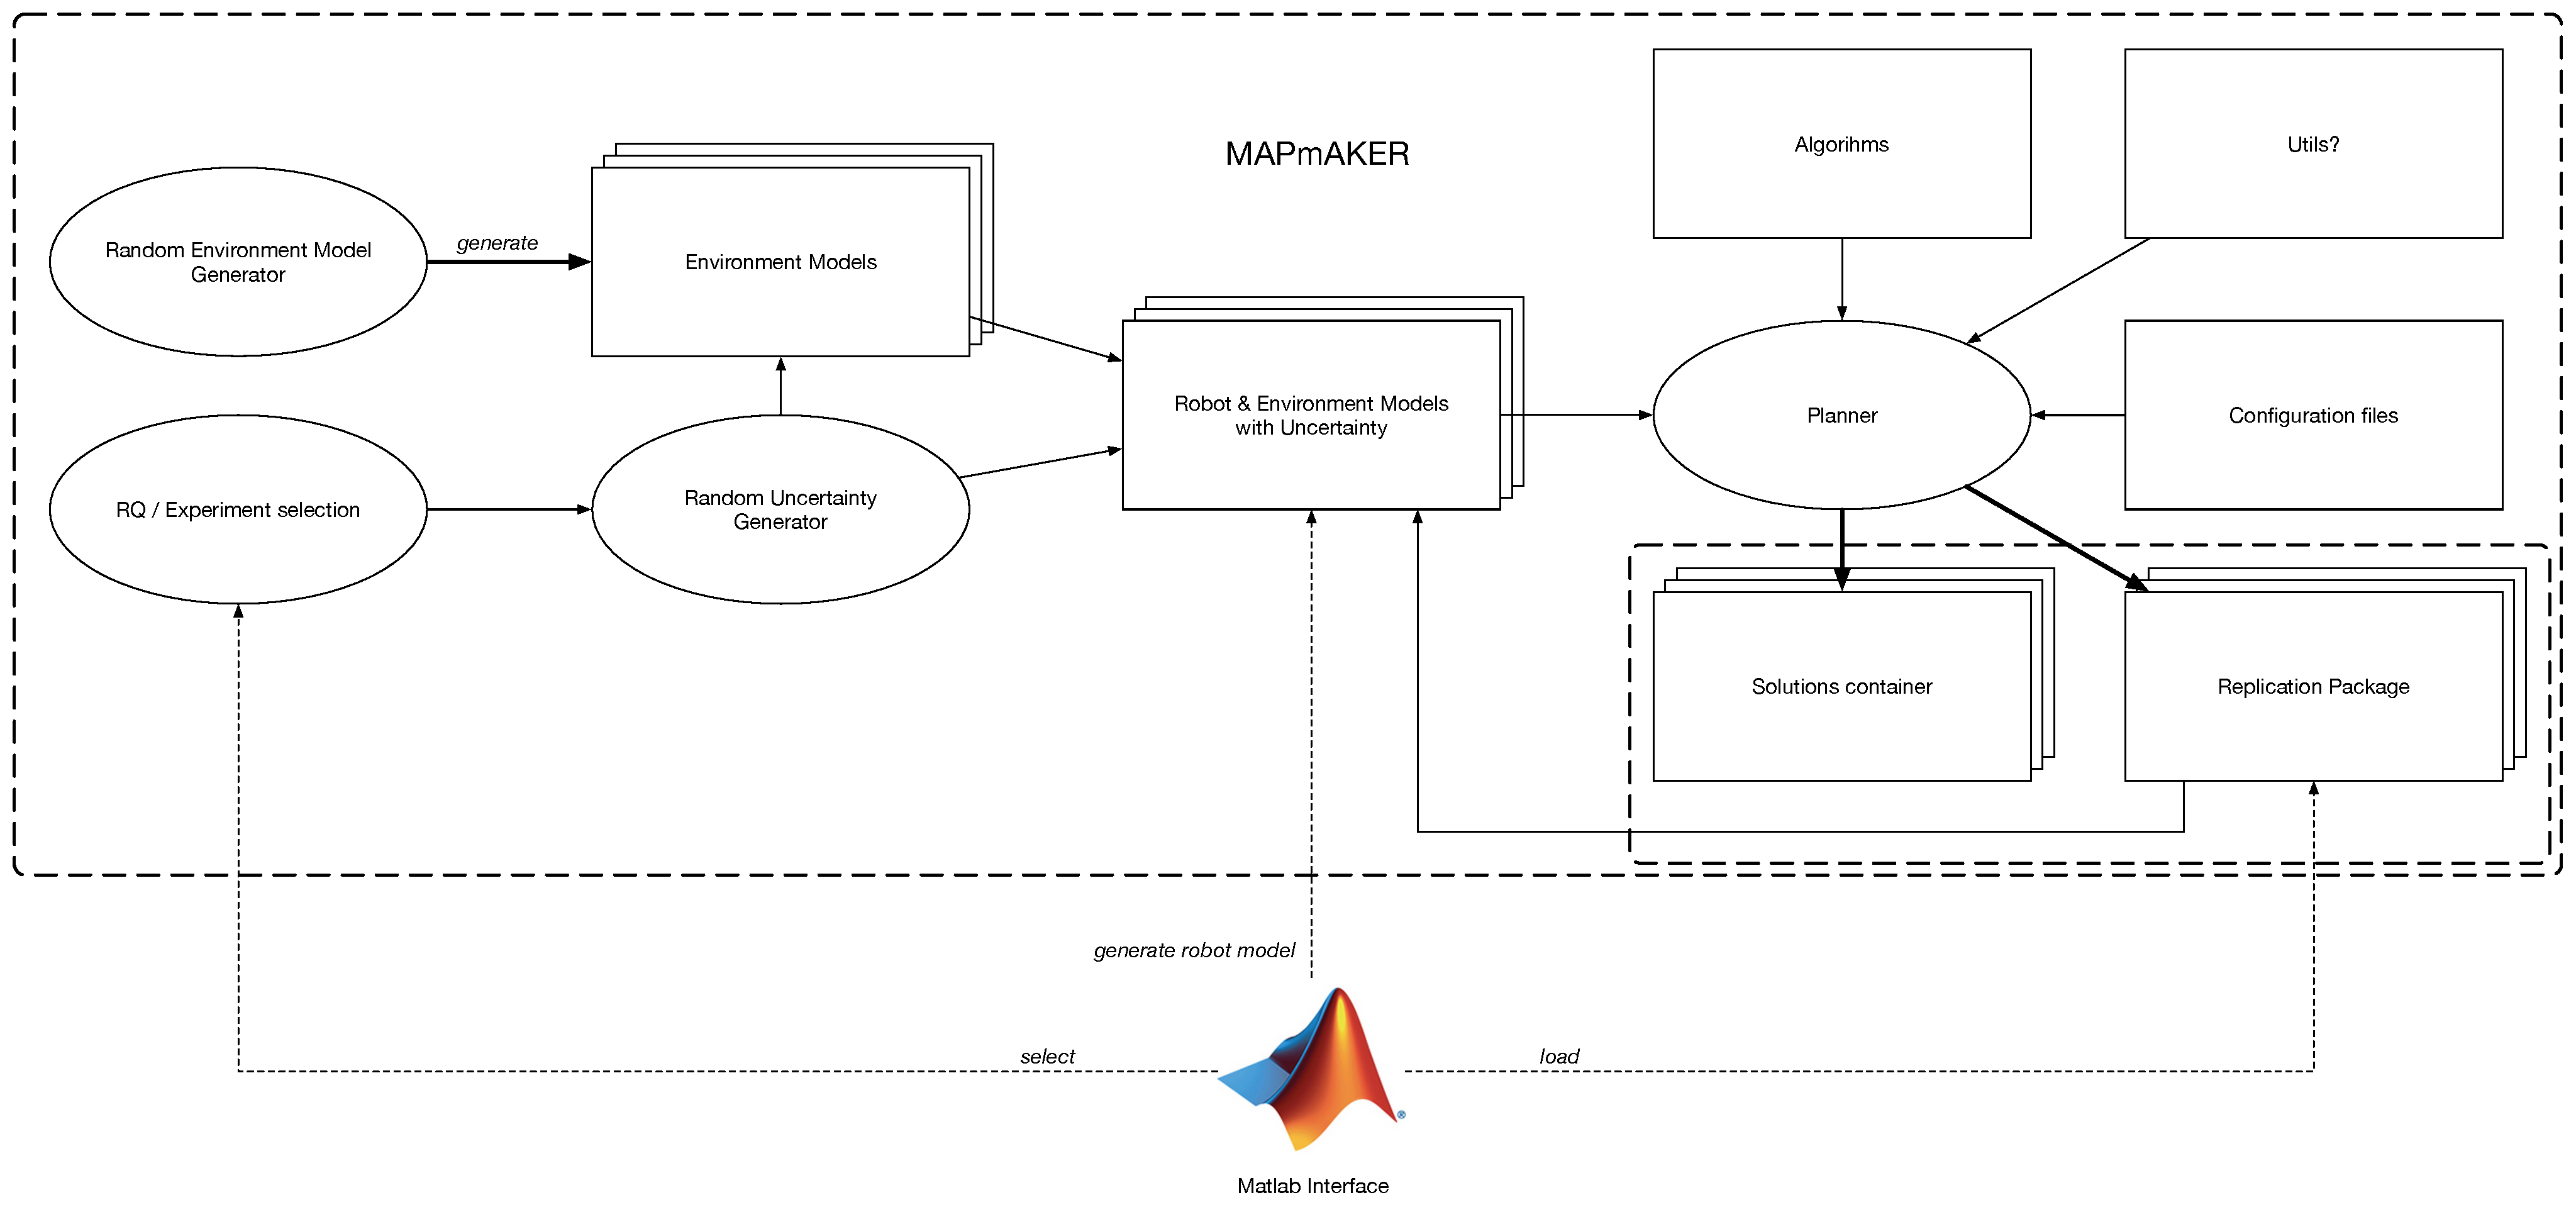
\includegraphics[width=1\linewidth]{Figures/MAPmAKER.pdf}
\caption{Overview of the MAPmAKER approach.}
\label{fig:overview}
\end{center}
\end{figure}





